%%%%%%%%%%%%%%%%%%%%%%%%%%%%%%%%%%%%%%%%%
% Programming/Coding Assignment
% LaTeX Template
%
% This template has been downloaded from:
% http://www.latextemplates.com
%
% Original author:
% Ted Pavlic (http://www.tedpavlic.com)
%
% Note:
% The \lipsum[#] commands throughout this template generate dummy text
% to fill the template out. These commands should all be removed when 
% writing assignment content.
%
% This template uses a Perl script as an example snippet of code, most other
% languages are also usable. Configure them in the "CODE INCLUSION 
% CONFIGURATION" section.
%
%%%%%%%%%%%%%%%%%%%%%%%%%%%%%%%%%%%%%%%%%

%----------------------------------------------------------------------------------------
%	PACKAGES AND OTHER DOCUMENT CONFIGURATIONS
%----------------------------------------------------------------------------------------

\documentclass{article}

\usepackage{fancyhdr} % Required for custom headers
\usepackage{lastpage} % Required to determine the last page for the footer
\usepackage{extramarks} % Required for headers and footers
\usepackage[usenames,dvipsnames]{color} % Required for custom colors
\usepackage{graphicx} % Required to insert images
\usepackage{listings} % Required for insertion of code
\usepackage{courier} % Required for the courier font
\usepackage{lipsum} % Used for inserting dummy 'Lorem ipsum' text into the template
\usepackage{amsmath}
\usepackage{amssymb}
\usepackage{amsthm}
\usepackage{array}
\usepackage{xy}
\usepackage{enumerate}
\usepackage{tabstackengine}
\usepackage{subfigure}
\stackMath
\usepackage{caption}

\usepackage[table]{xcolor}

% Margins
\topmargin=-0.45in
\evensidemargin=0in
\oddsidemargin=0in
\textwidth=6.5in
\textheight=9.0in
\headsep=0.25in

\linespread{1.1} % Line spacing

% Set up the header and footer
\pagestyle{fancy}
\lhead{\hmwkAuthorName} % Top left header
\chead{\hmwkClass\ : \hmwkTitle} % Top center head
\rhead{\firstxmark} % Top right header
\lfoot{\lastxmark} % Bottom left footer
\cfoot{} % Bottom center footer
\rfoot{Page\ \thepage\ of\ \protect\pageref{LastPage}} % Bottom right footer
\renewcommand\headrulewidth{0.4pt} % Size of the header rule
\renewcommand\footrulewidth{0.4pt} % Size of the footer rule

\setlength\parindent{0pt} % Removes all indentation from paragraphs

%----------------------------------------------------------------------------------------
%	CODE INCLUSION CONFIGURATION
%----------------------------------------------------------------------------------------

\renewcommand{\qedsymbol}{$\blacksquare$}

\definecolor{MyDarkGreen}{rgb}{0.0,0.4,0.0} % This is the color used for comments
\lstloadlanguages{Perl} % Load Perl syntax for listings, for a list of other languages supported see: ftp://ftp.tex.ac.uk/tex-archive/macros/latex/contrib/listings/listings.pdf
\lstset{language=Perl, % Use Perl in this example
        frame=single, % Single frame around code
        basicstyle=\small\ttfamily, % Use small true type font
        keywordstyle=[1]\color{Blue}\bf, % Perl functions bold and blue
        keywordstyle=[2]\color{Purple}, % Perl function arguments purple
        keywordstyle=[3]\color{Blue}\underbar, % Custom functions underlined and blue
        identifierstyle=, % Nothing special about identifiers                                         
        commentstyle=\usefont{T1}{pcr}{m}{sl}\color{MyDarkGreen}\small, % Comments small dark green courier font
        stringstyle=\color{Purple}, % Strings are purple
        showstringspaces=false, % Don't put marks in string spaces
        tabsize=5, % 5 spaces per tab
        %
        % Put standard Perl functions not included in the default language here
        morekeywords={rand},
        %
        % Put Perl function parameters here
        morekeywords=[2]{on, off, interp},
        %
        % Put user defined functions here
        morekeywords=[3]{test},
       	%
        morecomment=[l][\color{Blue}]{...}, % Line continuation (...) like blue comment
        numbers=left, % Line numbers on left
        firstnumber=1, % Line numbers start with line 1
        numberstyle=\tiny\color{Blue}, % Line numbers are blue and small
        stepnumber=5 % Line numbers go in steps of 5
}

% Creates a new command to include a perl script, the first parameter is the filename of the script (without .pl), the second parameter is the caption
\newcommand{\perlscript}[2]{
\begin{itemize}
\item[]\lstinputlisting[caption=#2,label=#1]{#1.pl}
\end{itemize}
}

%----------------------------------------------------------------------------------------
%	DOCUMENT STRUCTURE COMMANDS
%	Skip this unless you know what you're doing
%----------------------------------------------------------------------------------------

% Header and footer for when a page split occurs within a problem environment
\newcommand{\enterProblemHeader}[1]{
\nobreak\extramarks{#1}{#1 continued on next page\ldots}\nobreak
\nobreak\extramarks{#1 (continued)}{#1 continued on next page\ldots}\nobreak
}

% Header and footer for when a page split occurs between problem environments
\newcommand{\exitProblemHeader}[1]{
\nobreak\extramarks{#1 (continued)}{#1 continued on next page\ldots}\nobreak
\nobreak\extramarks{#1}{}\nobreak
}

\setcounter{secnumdepth}{0} % Removes default section numbers
\newcounter{homeworkProblemCounter} % Creates a counter to keep track of the number of problems

\newcommand{\homeworkProblemName}{}
\newenvironment{homeworkProblem}[1][Problem \arabic{homeworkProblemCounter}]{ % Makes a new environment called homeworkProblem which takes 1 argument (custom name) but the default is "Problem #"
\stepcounter{homeworkProblemCounter} % Increase counter for number of problems
\renewcommand{\homeworkProblemName}{#1} % Assign \homeworkProblemName the name of the problem
\section{\homeworkProblemName} % Make a section in the document with the custom problem count
\enterProblemHeader{\homeworkProblemName} % Header and footer within the environment
}{
\exitProblemHeader{\homeworkProblemName} % Header and footer after the environment
}

\newcommand{\problemAnswer}[1]{ % Defines the problem answer command with the content as the only argument
\noindent\framebox[\columnwidth][c]{\begin{minipage}{0.98\columnwidth}#1\end{minipage}} % Makes the box around the problem answer and puts the content inside
}

\newcommand{\homeworkSectionName}{}
\newenvironment{homeworkSection}[1]{ % New environment for sections within homework problems, takes 1 argument - the name of the section
\renewcommand{\homeworkSectionName}{#1} % Assign \homeworkSectionName to the name of the section from the environment argument
\subsection{\homeworkSectionName} % Make a subsection with the custom name of the subsection
\enterProblemHeader{\homeworkProblemName\ [\homeworkSectionName]} % Header and footer within the environment
}{
\enterProblemHeader{\homeworkProblemName} % Header and footer after the environment
}

%----------------------------------------------------------------------------------------
%	NAME AND CLASS SECTION
%----------------------------------------------------------------------------------------

\newcommand{\hmwkTitle}{Problem Set\ \#1} % Assignment title
\newcommand{\hmwkDueDate}{December 22, 2015} % Due date
\newcommand{\hmwkClass}{MLND} % Course/class
\newcommand{\hmwkClassTime}{} % Class/lecture time
\newcommand{\hmwkClassInstructor}{} % Teacher/lecturer
\newcommand{\hmwkAuthorName}{Jonathan Li} % Your name

%----------------------------------------------------------------------------------------
%	TITLE PAGE
%----------------------------------------------------------------------------------------

\title{
\vspace{2in}
\textmd{\textbf{\hmwkClass:\ \hmwkTitle}}\\
\normalsize\vspace{0.1in}\small{Due\ on\ \hmwkDueDate}\\
%\vspace{0.1in}\large{\textit{\hmwkClassInstructor\ \hmwkClassTime}}
\vspace{3in}
}

\author{\textbf{\hmwkAuthorName}}
\date{} % Insert date here if you want it to appear below your name

%----------------------------------------------------------------------------------------

\begin{document}

\maketitle

%----------------------------------------------------------------------------------------
%	TABLE OF CONTENTS
%----------------------------------------------------------------------------------------

%\setcounter{tocdepth}{1} % Uncomment this line if you don't want subsections listed in the ToC

%\newpage
%\tableofcontents
\newpage

%----------------------------------------------------------------------------------------
%	PROBLEM 1
%----------------------------------------------------------------------------------------

% To have just one problem per page, simply put a \clearpage after each problem
\begin{homeworkProblem}
		Statistics describing the housing prices and features are shown below. 
		\begin{center}
			\begin{tabular}{| l | l |}
				\hline
				Size of data & 506 \\ \hline
				Number of features & 13 \\ \hline
				Minimum price & 5.0 \\ \hline
				Maximum price & 50.0 \\ \hline
				Mean price & 22.5 \\ \hline
				Median price & 21.2 \\ \hline
				Standard dev. & 9.2 \\ \hline
			\end{tabular}
		\end{center}
\end{homeworkProblem}


\begin{homeworkProblem}

	\begin{itemize}
		\item 
		\textit{Which measure of model performance is best to use for predicting Boston housing data and analyzing the errors? Why do you think this measurement most appropriate? Why might the other measurements not be appropriate here?}
		
		I chose the mean absolute error as my model performance metric. MAE is not as sensitive to outliers as a mean squared error metric. When using MSE, there appeared to be a peak in error when using a training size of ~175 and a depth of 7 seen in Fig. ~\ref{peak}. I suspected that this may have been the result of an outlier in the training set. Indeed, when I plotted squared errors between actual and predicted prices generated by the best-fit parameters, an outlier appears at ~175 in Fig. ~\ref{outlier}. Thus, to account for outliers, I chose to use a MSE metric. 
		
		\begin{figure}[ht!] 
		   \centering
		   \subfigure[]{
		   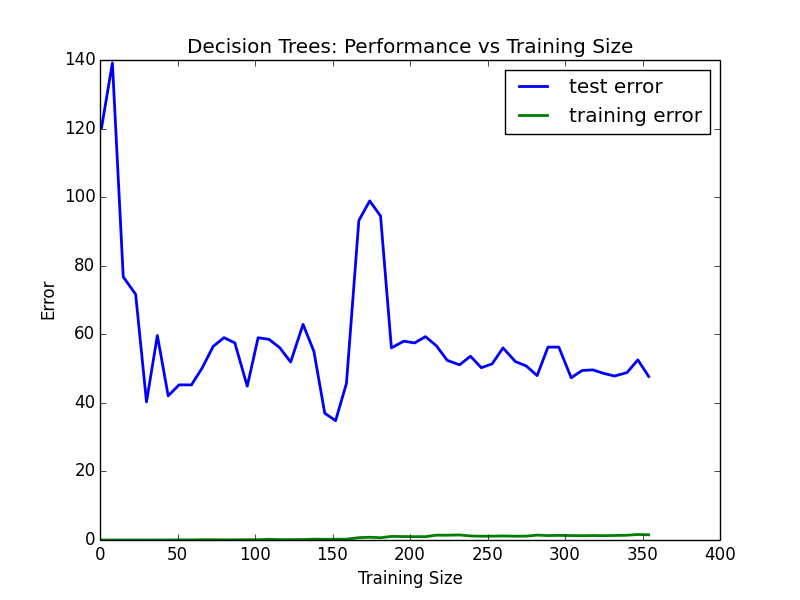
\includegraphics[width=2.5in]{figs/peak.png} 
		   \label{peak}
		   }
		   \subfigure[]{
		   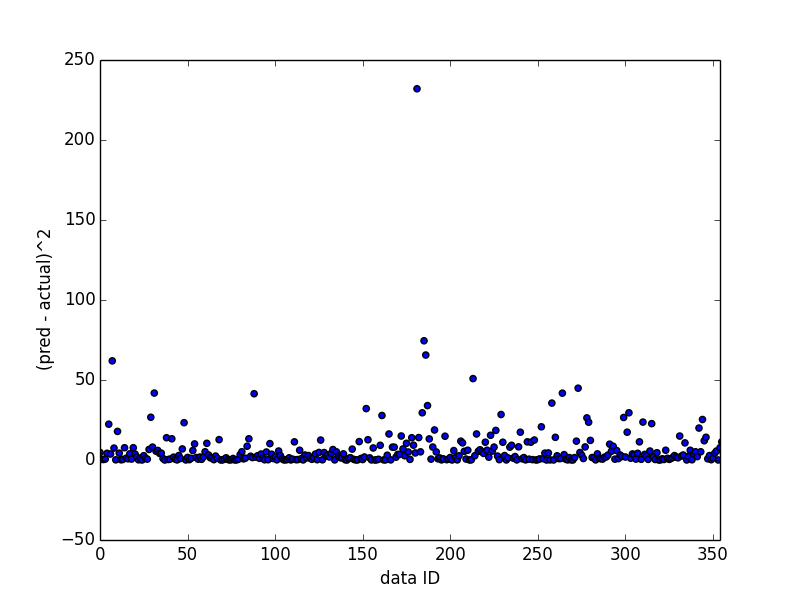
\includegraphics[width=2.5in]{figs/outlier.png} 
		   \label{outlier}
		   }
		   \caption{(a) A peak in test error is observed at a training size of ~175. (b) An outlier is found at roughly the same location in the data. }
		\end{figure}
		
		\item
		\textit{Why is it important to split the Boston housing data into training and testing data? What happens if you do not do this?}
		
		The training data is clearly necessary to build a model. However, if we used all the Boston housing data to train the model, then we would not have any data left over to test how well the model performs. Furthermore, using some of the training data as testing data is not an option either, as this would not give us any indication about the predictive power of the model.
		
		\item 
		\textit{What does grid search do and why might you want to use it?}
		
		The fit of a model can depend greatly on its input parameters. For instance, Fig. 2 shows that the depth of a decision tree can greatly affect training and test errors. The grid search allows us to test a space of one or more parameters to find the best fit model. 
		
		\begin{figure}[ht!] 
		   \centering
		   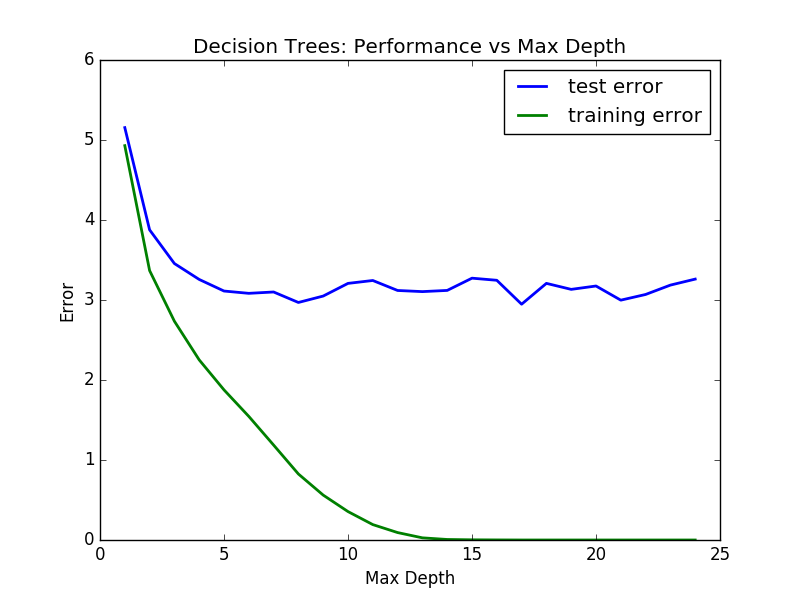
\includegraphics[width=4in]{figs/depth_error.png} 
		   \label{depth_error}
		   \caption{Training and test errors decrease with increasing depth, but hit a plateau at around 5. }
		\end{figure}

		\item
		\textit{Why is cross validation useful and why might we use it with grid search?}
		
		Cross validation is useful because it allows us to use all the data available for both training and testing. This allows us to maximize accuracy, since we do not have to worry as much about biased sampling of the data set. We would especially want to use it for grid search because we are testing different model parameters against each other, and need a more accurate score to determine their performances
		
	\end{itemize}
\end{homeworkProblem}


\begin{homeworkProblem}
	\begin{itemize}
		\item
		\textit{Look at all learning curve graphs provided. What is the general trend of training and testing error as training size increases?}
		
		The general trend is that training error increases gradually as training size increases, which is to be expected. However, the testing error initially decreases sharply, and plateaus quite quickly. This suggests that a good model could be created from a small sample size, and adding more data does not necessarily refine the model any further. 
		
		\item
		\textit{Look at the learning curves for the decision tree regressor with max depth 1 and 10 (first and last learning curve graphs). When the model is fully trained does it suffer from either high bias/underfitting or high variance/overfitting?}
		
		It appears that the models suffer from underfitting with the max depth is too small, as the error remains high. A model that is too simplistic may not be able to capture the important features of the data, and thus would not be able to accurately predict the test data. When we use a max depth of 10 (Figure 3(b)), we observe classic overfitting. In particular, the training error is much less than the test error, so the model does not generalize well to test data. 
		
\begin{figure}[ht!] 
		   \centering
		   \subfigure[]{
		   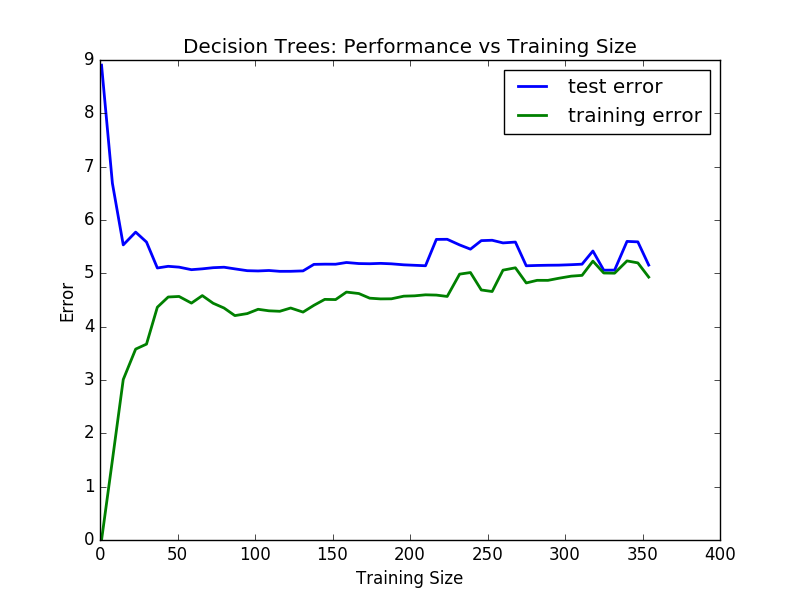
\includegraphics[width=2.5in]{figs/depth_1.png} 
		   \label{peak}
		   }
		   \subfigure[]{
		   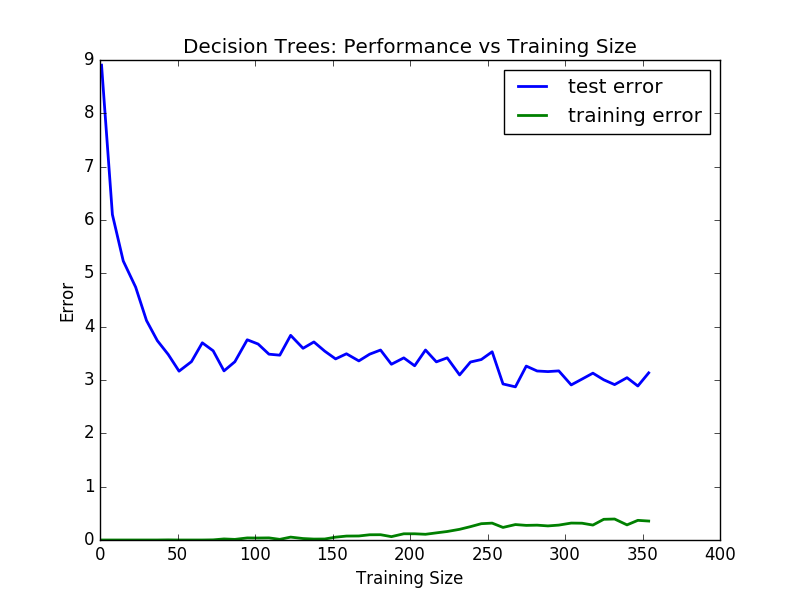
\includegraphics[width=2.5in]{figs/depth_10.png} 
		   \label{outlier}
		   }
		   \caption{Errors for test (blue) and training (green) errors for varying sample sizes for a maximum depth of (a) 1 and (b) 10. }
		\end{figure}
				

		\item
		\textit{Look at the model complexity graph. How do the training and test error relate to increasing model complexity? Based on this relationship, which model (max depth) best generalizes the dataset and why?}
		
		Fig. 2 shows that the test error reaches a stable minimum at a max depth of around 5. This suggests that the model generalizes well at a max depth of 5, since higher depths do not seem do decrease error. We note that training error also decreases with max depth, but at a slower rate. As expected, training error will eventually reach 0, as each leaf will eventually contain a singlet data point. However, we would prefer smaller trees due to space and time considerations. 
	\end{itemize}
\end{homeworkProblem}

\begin{homeworkProblem}
	\begin{itemize}
		\item
		\textit{Model makes predicted housing price with detailed model parameters (max depth) reported using grid search. Note due to the small randomization of the code it is recommended to run the program several times to identify the most common/reasonable price/model complexity.}
		
		The best fit decision tree model predicts an average price of 20.3 and a depth of 6. 
		
		\item 
		\textit{Compare prediction to earlier statistics and make a case if you think it is a valid model.}
		
		The sample to be predicted is very similar to data point 470 which has the features 
		
		\texttt{[12.05, 0.0,18.10,0,0.61,5.65, 87.6, 1.95,24,666,20.2, 291.55,14.10,20.8]}
		
		and has a price of 20.8. Furthermore, an analysis of the 10 nearest neighbors show the average price is 21.52, which is close to the prediction. In addition, the prediction is well within the range of one standard deviation from the mean price, and is also close to the median. 

	\end{itemize}
\end{homeworkProblem}

%----------------------------------------------------------------------------------------

\end{document}